\section{Network Fusion}
To be able to combine iris and face verification, a combination of the results of the two networks can be made.  This is done by having two individual streams that are merged at their last \gls{fc} layer by concatenating the layers along their longest dimension. The merged layer can then be fed into other \gls{fc} layers and further to a classification layer. This can be done using a softmax layer after the \gls{fc} layer \citep{Eitel2015}. This should in theory increase the accuracy in ID verification in a potential instance where verification is required. The architecture used is shown in \autoref{fig:net_fusion}. The two \gls{fc} had 5020 neurons to have the same dimensions as the concatenated layer. To see if the new merged structure performs better than the iris and face \gls{cnn}s separately, the same hyper parameters are used as in \autoref{sec:cnn_iris_rec}.

%To be able to reuse as much as possible, the two databases used with the networks separately are also used in the fusion of the networks instead of using a multimodal database as presented in \autoref{cha:Research}. This means that a combination of the two databases is necessary as the data have not been collected by the same groups or from the same people. The databases does not have the same amount of classes, therefore the larger database is reduced also reducing the entire amount of usable data.

\subsection{Multimodal Database}
The fusion net should be trained with a multimodal biometric database. Ideally the database used in this project should consist of face and iris images obtained from the same subjects captured with the same camera complying with the requirements set in \autoref{ch:req}. 

However, even though literature suggests that chimeric databases are less adequate than genuine multimodal biometric databases, the multimodal database used during the work with information fusion is synthetically created. As \autoref{sec:multi_modal_data} mentions there are only a limited amount of multimodal biometric databases available containing both iris and face data, and to the extend of the knowledge gained from the research presented in \autoref{sec:info_fuse} there is only one of the databases which is obtained using mobile devices namely the MobBio database. For this database the Asus Transformer Pad TF 300T is used, which has a camera of 8MP, which is comparable to the iPhone 5s used for the caption of the Warsaw-BioBase used for the iris identification methods presented in \autoref{BasicM} and \autoref{sec:cnn_iris_rec} \citep{Sequeira2014}. However, despite several attempts of contacting the authors of the database it was not possible to establish communication or gain access to the database. Therefore the available way to obtain a multimodal database with mobile device images is to create it synthetically. Furthermore as the goal is to compare the performance of the fused \gls{cnn}s with the individual \gls{cnn}s on the face and iris data respectively, it is desirable to test on the same data. Therefore a databased was created by combining the \gls{lfw} and the Warsaw-BioBase. 

The database was created by combining iris classes arbitrarily with an face class for as many classes as there were classes available from both the iris and the face dataset. Before combining the datasets the classes with ten or less samples were discarded. The new samples were made by giving the iris image and the face image the same label. The new samples were then data augmented as described in \autoref{sec:cnn_iris_rec}

\subsection{Results}
The chimera database consists of 20640 samples across 91 classes. 70\% was used for training, 15\% for validation and 15\% for testing. The network was trained for 140 epochs and achieved a test accuracy of 81.17\%

\begin{figure}[H]
	\centering
	\begin{subfigure}{0.48\textwidth}
		\centering
		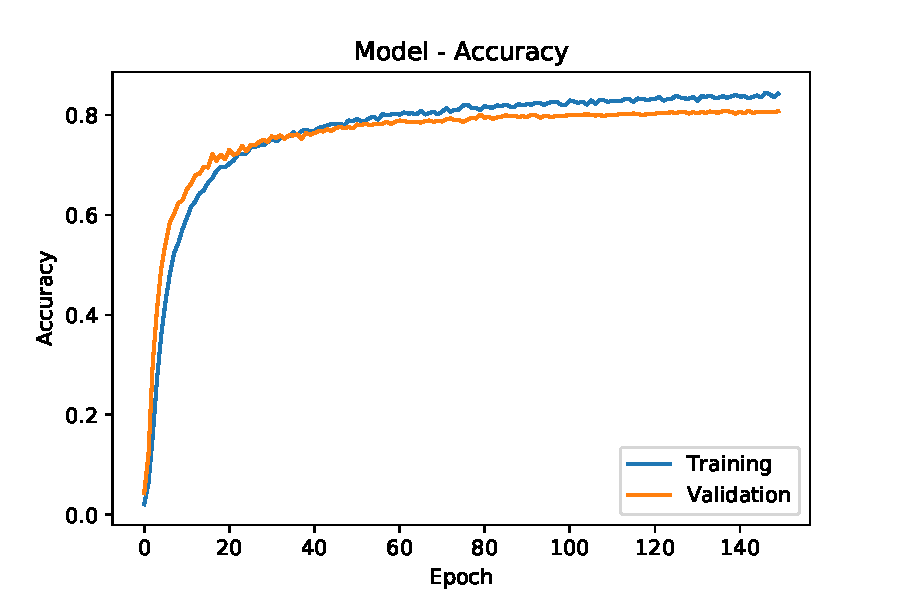
\includegraphics[width=\textwidth]{merged_acc_81_17_acc}
		\caption{Face recognition \gls{cnn} accuracy progression through epochs}
		\label{fig:merged_acc}
	\end{subfigure}
	\begin{subfigure}{0.48\textwidth}
		\centering
		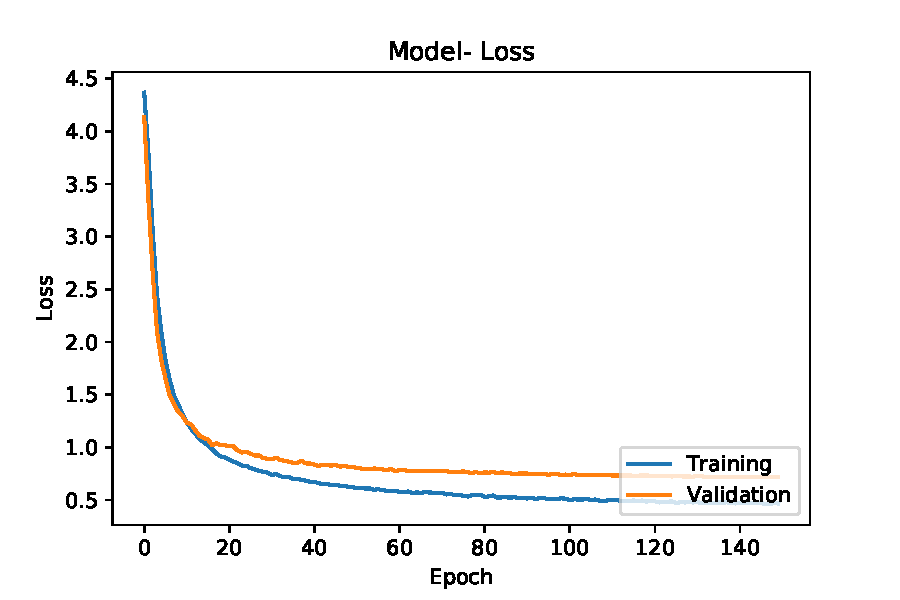
\includegraphics[width=\textwidth]{merged_acc_81_17_loss}
		\caption{Face recognition \gls{cnn} loss progression through epochs}
		\label{fig:merged_loss}
	\end{subfigure}
	\caption{Accuracy and loss progression for the merged \gls{cnn}. Achieved 81.17\% accuracy on the test set}
	\label{fig:merged_graphs}
\end{figure}

\noindent As the merged \gls{cnn} using the chimera data performed worse by almost 20\% something was wrong. To investigate how the separate iris and face \gls{cnn}s would perform on the chimera data a second test was made. This was done by simply discarding either the iris or the face respectively from the generated sample. This produced the following result with the same 70, 15, 15 split.  The iris \gls{cnn} achieved 68.94\% accuracy on the test set, \autoref{fig:iris_cnn_68_graphs}. The VGG face \gls{cnn} achieved 77.78\% accuracy on the test set, \autoref{fig:vgg_77_graphs}. When all networks used the same data the merged network seems to outperform both the VGG face \gls{cnn} and the iris \gls{cnn} although they both achieved above 99\% accuracy when trained on the data before the it was fused to the chimera data.

\begin{figure}[H]
	\centering
	\begin{subfigure}{0.48\textwidth}
		\centering
		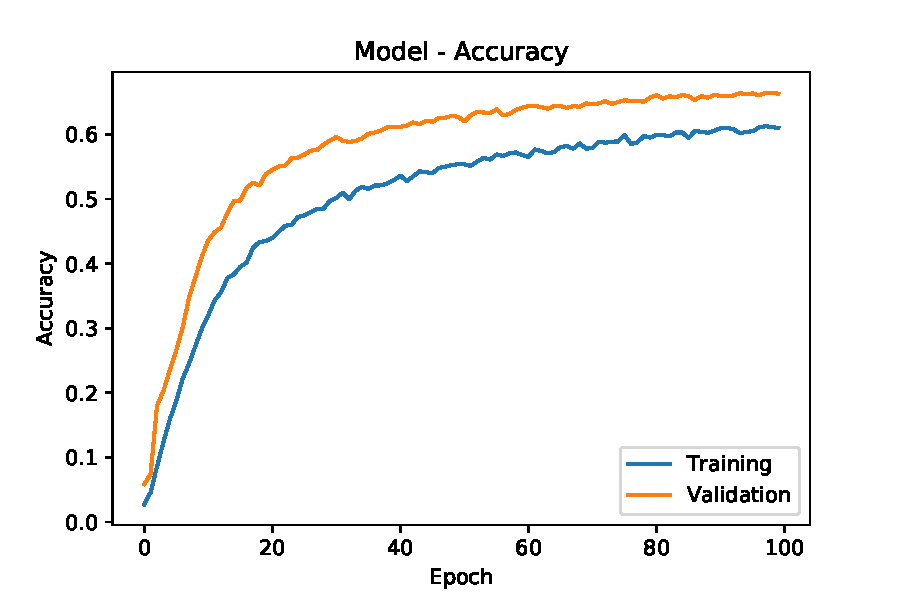
\includegraphics[width=\textwidth]{iris_cnn_bad_68_94_acc}
		\caption{Iris \gls{cnn} accuracy progression through epochs}
		\label{fig:iris_cnn_68_acc}
	\end{subfigure}
	\begin{subfigure}{0.48\textwidth}
		\centering
		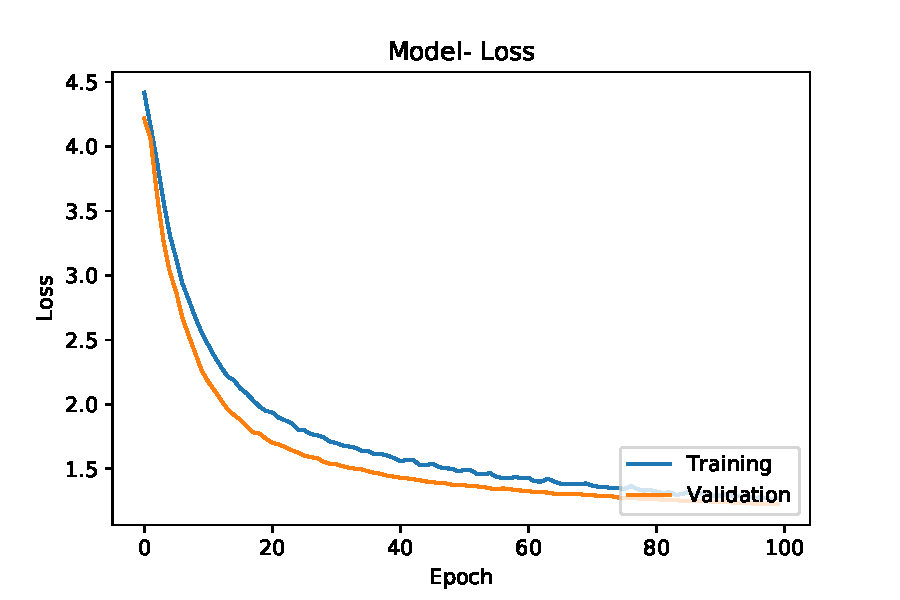
\includegraphics[width=\textwidth]{iris_cnn_bad_68_94_loss}
		\caption{Iris \gls{cnn} loss progression through epochs}
		\label{fig:iris_cnn_68_loss}
	\end{subfigure}
	\caption{Accuracy and loss progression for the iris \gls{cnn} trained on chimera data. Achieved 68.94\% accuracy on the test set.}
	\label{fig:iris_cnn_68_graphs}
\end{figure}


\begin{figure}[H]
	\centering
	\begin{subfigure}{0.48\textwidth}
		\centering
		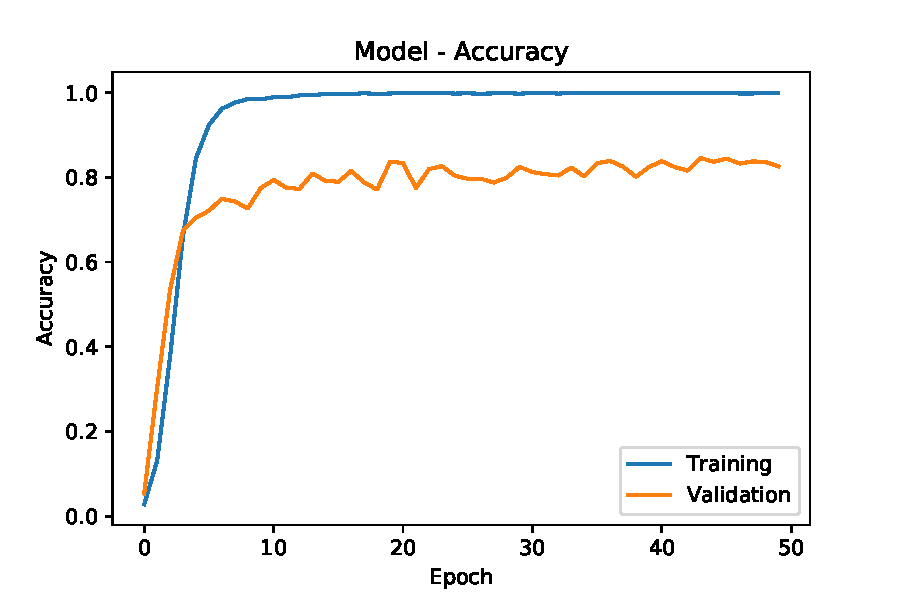
\includegraphics[width=\textwidth]{vgg16_bad_77_88_acc}
		\caption{Face recognition \gls{cnn} accuracy progression through epochs}
		\label{fig:vgg_77_acc}
	\end{subfigure}
	\begin{subfigure}{0.48\textwidth}
		\centering
		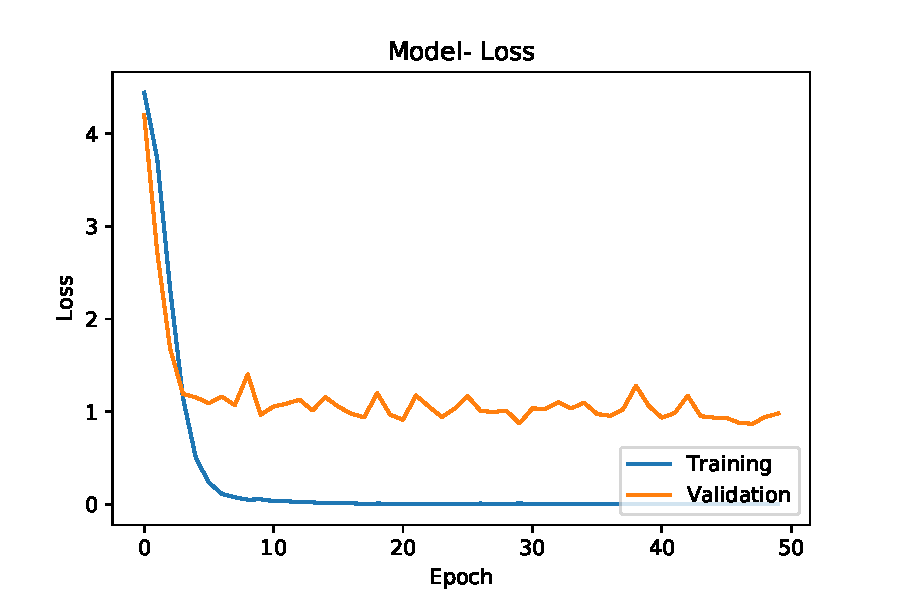
\includegraphics[width=\textwidth]{vgg16_bad_77_88_loss}
		\caption{Face recognition \gls{cnn} loss progression through epochs}
		\label{fig:vgg_77_loss}
	\end{subfigure}
	\caption{Accuracy and loss progression for the VGG face \gls{cnn} trained on chimera data. Achieved 77.78\% accuracy on the test set }
	\label{fig:vgg_77_graphs}
\end{figure}

